\chapter
{Creating and Interlinking Semantic Data on the Desktop with SemNotes}
\label{ch:semnotes}

\begin{flushright}
 \textit{Based on ``The Semantic Desktop at Work: Interlinking Notes'' \cite{Dragan2011a}\\published at the 7th International Conference on Semantic Systems (I-SEMANTICS~2011)}
\end{flushright}

The Semantic Desktop has been proposed as a solution to the ever growing problem of information overload on our computers. It provides the foundations necessary to integrate and manage personal information. However, the challenge of designing and realising semantic applications that use this infrastructure still remains. 
In this chapter, we present SemNotes\footnote{\url{http://smile.deri.ie/projects/semn}}, a semantic note-taking tool for the Nepomuk-KDE Semantic Desktop, as a tool for creating new semantic information on the desktop and integrating it seamlessly in the existing network of linked desktop data.
SemNotes provides a real-world, functional use case for fully exploiting the capabilities of the Semantic Desktop: interlinking, organisation and management of personal information, improved search and browsing. 
Furthermore, it represents our solution to a set of identified generic challenges for applications on the Semantic Desktop, as described by the first research question in Section \ref{sub:question}.
We describe a task-based user evaluation comparing SemNotes with a conventional note-taking tool. The results show that complex searches on interlinked information created with SemNotes are significantly faster, with little or no extra effort required from the users. 

\section{Introduction}
\label{sec:semnotesintro}

The Semantic Desktop provides a framework for creating applications and tools that simplify the daunting tasks of managing personal information accumulated on the desktop. 
The information overload problem, combined with the disconnection of data caused by application silos, is solved by the use of Semantic Web standards for storing and interlinking the desktop information. 
Data which before was stored separately by different applications can be now explicitly connected. The result is a network of interlinked personal information, which can be browsed by association, filtered and searched in a unified way. 

The Semantic Desktop overcomes the limitations of conventional desktops, where information is kept in different formats and application repositories, by using common vocabularies to describe the data, and a desktop-central place to store it, in a standardised format, accessible to all applications.

Indeed, the Semantic Desktop makes the information load manageable. However, new challenges emerge: one such new issue is how to design and realise semantic applications that use the infrastructure provided by the Semantic Desktop. We address this problem by dividing it into smaller, simpler challenges and providing solutions for each of them. To illustrate the solutions, we describe the design of a semantic note-taking application for the Nepomuk-KDE Semantic Desktop, called SemNotes. We use note-taking as an example because it is a desktop activity that is not limited to a specific domain, since the notes can widely vary in topic. It is also a common activity that plays an important role in Personal Information Management and that we believe would benefit from the use of semantic technologies.

\subsection{Challenges}
\label{sub:appchallenges}

In Section \ref{sub:question} we broke down the first research question \textbf{Q 1.}: \emph{How to build semantic applications and tools for the Semantic Desktop as to provide the best experience for the users, while creating reusable semantic data?}, into several sub-questions.
These are the challenges we found in designing new semantic applications for the Semantic Desktop:

\begin{description}
 \item[Q 1.1.] \emph{How to create semantic data that is correct, and maximises the reuse of existing Semantic Desktop data through interlinking?}\\
Applications should be aware of the data that is available on the desktop, from other applications. The data they produce is also accessible to other applications, and this should also be taken into account, because it raises the dual challenge of making sure that the data is represented correctly so that other applications can use it if they choose, as well as making the most of existing information through reuse and link creation. How to interlink information items is the most important challenge for adhering to the Semantic Desktop requirements of creating and maintaining a network of linked desktop data. It refers in the first place to the new information coming into the desktop through the application, and how to integrate it with the linked information that exists on the desktop. But it also covers the situation when the only new information created is in fact a new link between existing entities. 
Existing desktop data is heterogeneous. The reasons for this include the fact that different parts of it are created by different applications, with different functionalities and needs. So, although represented in a standardised way, the data is not always consistent, up-to-date or even correct. Furthermore, the data is also heterogeneous in terms of form: there are new types of information available to be integrated (i.e. tags, relations). Best practices advise the reuse of as much of the existing information as possible, because through reuse, the interlinking becomes deeper and richer. However, the possibility of reusing vast amounts of existing data raises other challenges, in selecting the right amount of necessary information for maximum benefit for the users, while not overloading them. The selection is complemented by the way the information is shown.
 \item[Q 1.2.] \emph{How to design the human-computer interaction in an application for the Semantic Desktop?}\\
This question relates to designing interfaces which support the existing workflow of the user, while integrating the additional semantic information in a useful way. A balance must be found between too much information, so that it interferes with the user doing tasks, and too little, or not enough to make a difference. The question also refers to more than just displaying the information in an interface --- allowing users to interlink information items easily, and generally aiding the creation of new semantic data is also a challenge for application development. Extra difficulty is added by the variety of interlinked information available on the desktop, combined with the reduced control of developers over what resources are linked from other tools.
 \item[Q 1.3.] \emph{How to correctly evaluate a semantic application?}\\
A challenge related to evaluation is the lack of a standardised dataset to use, due to the highly personal data required. Even if such a dataset existed, due to the fact that the applications on the Semantic Desktop are mainly related to personal information, it is difficult for participants to use the data provided, as they are not familiar with it. Evaluating PIM tools has been shown to yield best results when the test users are asked to perform their own tasks in their own set-up rather than attempting to simulate it with artificial tasks and artificial data. The reduced number of semantic application in each area makes it difficult to evaluate a new tool against an existing established one, thus the best candidates for a comparative evaluation are conventional (i.e. not semantic) applications with similar functionality. While possibly re-demonstrating that indeed linked data is more useful, comparing a semantic and non-semantic application requires well thought metrics, as the semantic features that need 
evaluating have no direct counterparts against which to evaluate them. For task based evaluations, it is difficult to find a common set of tasks that both applications can perform. A solution is to choose general, high level tasks, but that influences the granularity of the results.
\end{description}


\section{Tackling the Challenges: The Design of SemNotes}
\label{sec:semnotesdesign}

We use our note-taking application, SemNotes, to describe the general principles we used for designing an application for the Semantic Desktop. Note-taking is a good general use case for the Semantic Desktop because the information contained in notes is not restricted to a specific domain. Personal notes are naturally connected to the user's context, and can thus be meaningfully interconnected with much of the existing network of personal data on the desktop.

We divided the design into specialised modules. Each module handles a set of related tasks. We describe the modules as they would be for a general semantic application, followed by a more specific description about the implementation of SemNotes in the next section.
 
\subsection{Data Representation} 

This module handles the vocabulary of the application: the \emph{data types} around which the application is centred, and the kind of \emph{metadata} that is needed for them. To enable other Semantic Desktop applications to understand the data produced, as well as for our application to understand data from the underlying Semantic Desktop, the best practice is to reuse existing desktop ontologies where possible. The basic data type handled by SemNotes is the note, represented by a short snippet of text containing personal information. 

\subsection{Data Management} 

This module manages the life-cycle of the semantic data that the application handles, by enabling the transition between the phases of the life-cycle. We adapted the Abstract Data Life-Cycle Model \cite{MoellerPhDThesis2009} to illustrate a comprehensive workflow for Semantic Desktop data, from its creation to its termination. Figure~\ref{fig:datalifecycle} shows the phases and transitions between them, focusing on the possible actions that the user can execute, and hence, that a semantic application could support.

\begin{figure}[htb]
 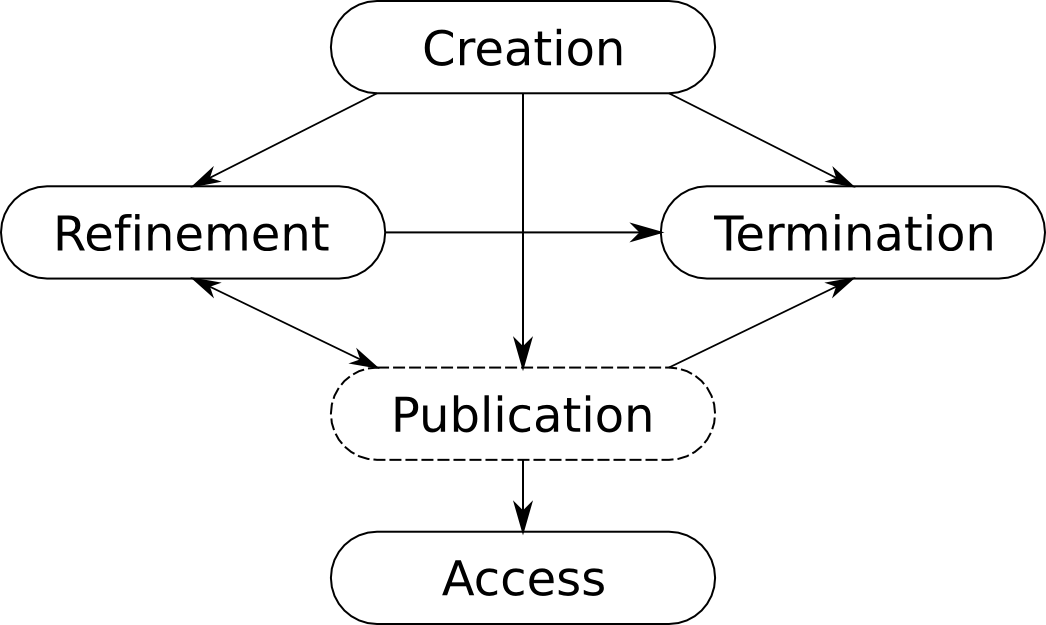
\includegraphics[width=0.7\linewidth]{chapters/core/img/lifecycle}
\caption{Semantic Desktop data life-cycle.}
\label{fig:datalifecycle}
\end{figure} 

\begin{description}
 \item[Creation.] Most often creation implies creating a new resource, of a given type. However, the import of existing data from other applications or formats (e.g. crawlers) is also included here.
 \item[Refinement.] This phase includes any activities that make changes to existing data. It also contains the creation and deletion of links between existing resources, although alternatively they can be included in the Creation or Termination phases, as links are data too. 
 \item[Access.] This phase is represented by accessing the data through either querying or browsing. Because we are discussing interlinked data, accessing a piece of semantic data implies recursively accessing the sub-graph of resources semantically related to it. How much of the sub-graph is traversed can vary, and further traversal by the user should be supported and encouraged. 
 \item[Termination.] In this phase the data is deleted from the system. As with the access phase, rules must be defined to determine how much of the dataset a deletion will affect---e.g. it might make sense to delete all the subtasks of a task when the parent is deleted, but not to delete the documents related to the task.
 \item[Publication.] This phase represents making the data accessible to users from outside the system. Also included here is exporting the data to other formats and applications. When handling semantic personal data, applications should ensure that sensitive data is well protected against unauthorised or accidental publication. 
\end{description}

Furthermore, this module handles where and how the data is stored. The Semantic Desktop provides the framework for storing semantic data, therefore it is best that the central desktop repository be used, when practical. This enables easier interlinking with the rest of the data. In the case of SemNotes, the notes and all the metadata about them are stored in the desktop repository. 

\subsection{Interlinking} 

The interlinking module is logically a sub-module of the Data management one, as it specifically manages a part of the refinement phase of the data life-cycle. However, because it is an important part of any semantic application, relating to the first two challenges listed in Section \ref{sub:appchallenges}, we describe it as a standalone module. The interlinking module effectively realises the goal of integrating the new semantic data into the pool of existing linked desktop data. The functionalities offered can vary from simple automatic linking of new resources to a specified context or to their author, to complex extraction and inference of new relations and resources.  This module provides the feature that sets SemNotes apart from other note-taking tools, the interlinking of the notes with the desktop resources mentioned in them. In our application, there are two sub-modules, that handle \begin{inparaenum}[(i)] \item entity recognition, and \item information extraction\end{inparaenum}, suggesting 
possible new connections to be created by the user.
 
\subsection{Visualisation} 

The visualisation module presents the data to the user in a simple, yet useful and versatile way. It addresses the third challenge listed above: designing the interface. Depending on the application, the visualisation can include \emph{aggregated} views on the data, and \emph{filters}. Faceted search \cite{Yee2003} has proven useful for semantic data, and it can be used to present the interlinked information to the user in a meaningful way. In SemNotes, the data that needs to be visualised is basically an enhanced version of a list of notes, with sorting and filtering. The module also provides the note editor. An important part of the module is displaying the recommendations for interlinking, a difficult task due to the heterogeneous nature of the information to be presented in a uniform, uncluttered way.

We describe how we tackled the last question --- the evaluation of the application --- in Section \ref{sec:semnotesevaluation}. 


\section{Implementation of SemNotes}
\label{sec:semnotesimplementation}

In the development of SemNotes, we tried to reuse as much as possible of the features provided by the host Semantic Desktop, Nepomuk-KDE\@. Using the existing functionality enabled better integration with the rest of the system, while reducing the effort required for the implementation. Nepomuk-KDE provides out of the box central RDF storage for the desktop, and an efficient means to access and query the data. 

We describe below the implementation of each of the modules introduced in the design section. 

\subsection{Data Representation} 
\label{sub:datarepresentation}

We describe the data created by SemNotes using a subset of the desktop ontologies described in Section \ref{sub:nepomuk} --- Personal Information Model (PIMO) and Nepomuk Annotation Ontology (NAO). 
Figure~\ref{fig:holiday} shows a basic note with metadata, and Listing \ref{lst:noterdf} contains the Turtle representation of the same example. 

The central unit of information handled by SemNotes is the note --- represented as an instance of \verb|pimo:Note|. 
The information stored for each note consists of: 
\begin{itemize}
 \item title --- \verb|nao:prefLabel|
 \item content --- \verb|nao:description|
 \item creation date --- \verb|nao:created|
 \item last modification date --- \verb|nao:lastModified|
 \item rating --- \verb|nao:numericRating|
 \item tags --- \verb|nao:hasTag|
 \item related desktop resources --- \verb|pimo:isRelated|
\end{itemize}

The Nepomuk ontologies make the distinction between resources representing native computer structures, which are described with the Nepomuk Information Element (NIE) ontology and resources representing concepts in the real world, which are described with the Personal Information Model (PIMO).

Before representing the PIMO concepts, most of the semantic data on the desktop is extracted from \verb|nie:DataObject|s and interpreted as \verb|nie:InformationElement|s. This is due to the fact that generally the information is still created by non-semantic applications, and to make it useful to the Semantic Desktop it has to be transformed, while keeping provenance information and feeding back into the applications that created it.

The extra step of extracting resources is not needed in the case of the information created directly for the Semantic Desktop by semantic applications. Thus, if no data is stored outside of the repository, no NIE resources are created. This is a characteristic of SemNotes and of other semantic applications for the Semantic Desktop.

The \verb|pimo:Note|s created with SemNotes can however be exported as text or HTML files, for backup or other purposes, thus associating a NIE resource to a note. This is the reverse of the usual process, and the change stems from working directly with the framework provided by the Semantic Desktop.

\begin{figure}[th]
 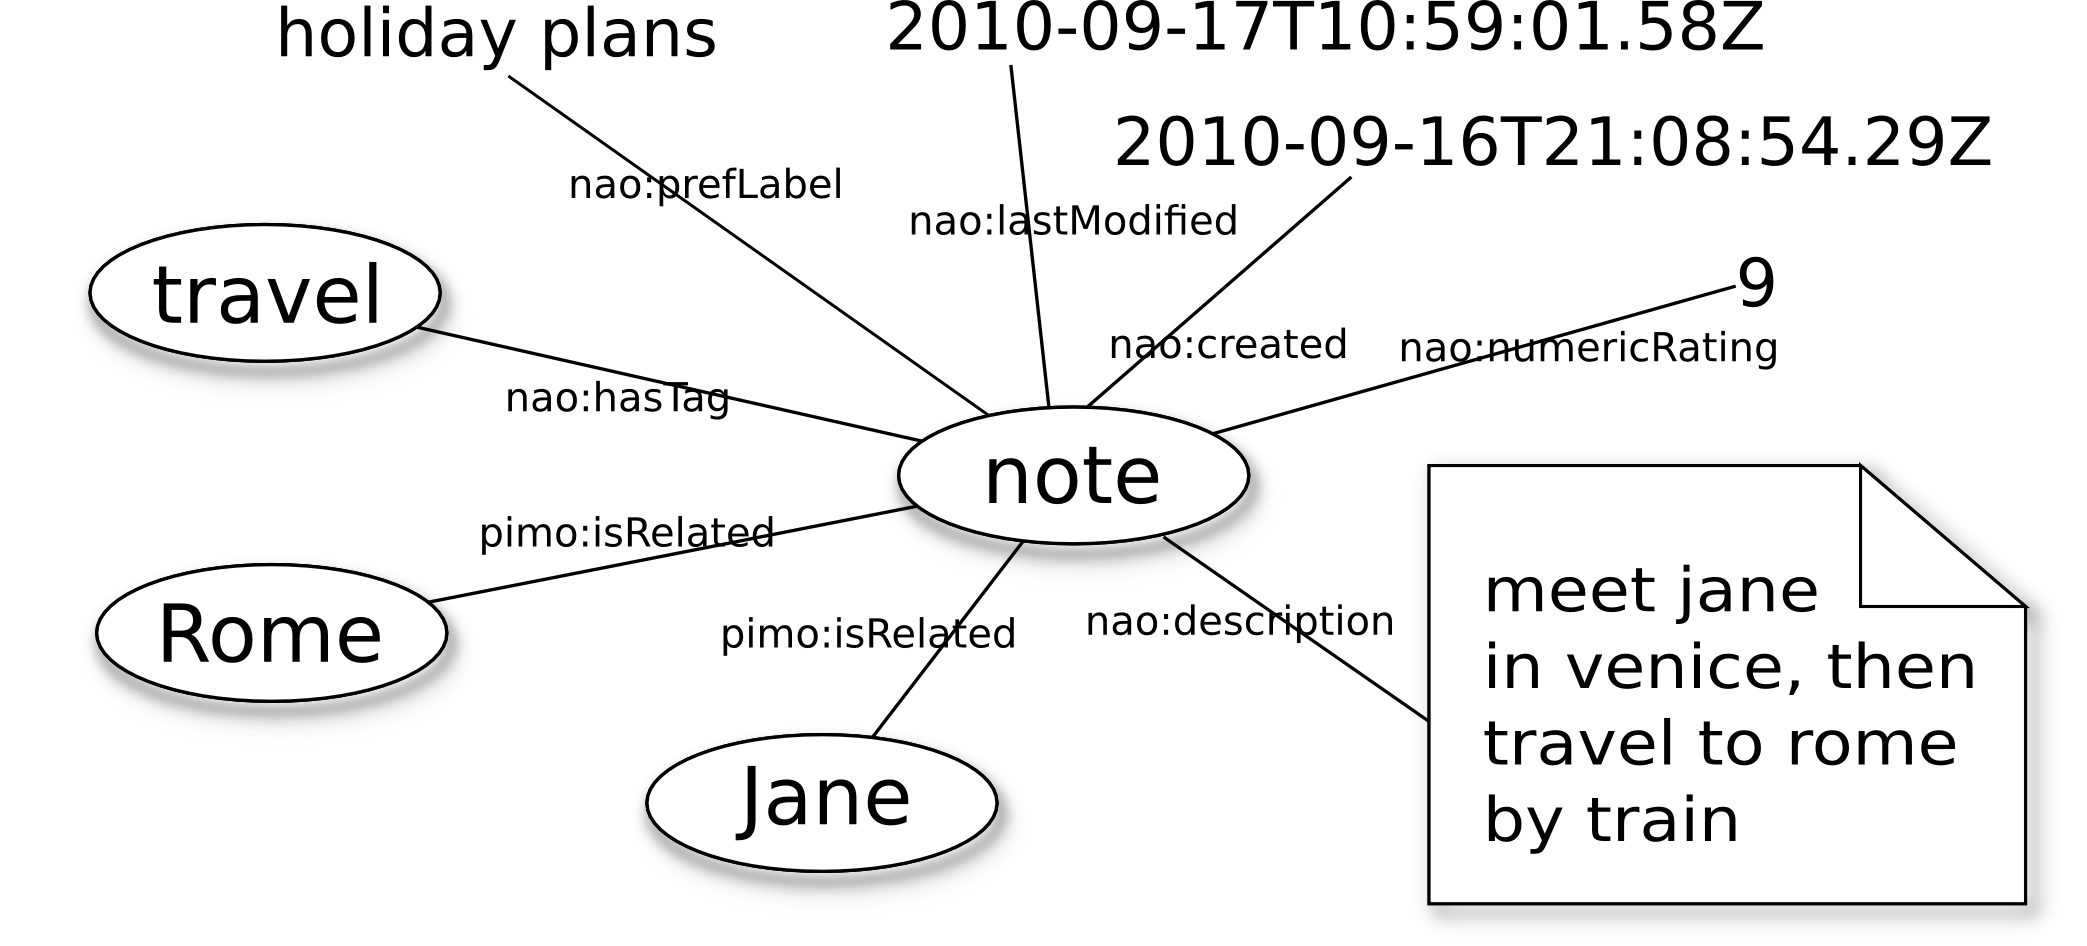
\includegraphics[width=0.9\linewidth]{chapters/core/img/note-properties}
\caption{Graph representation of the information about a note.}
\label{fig:holiday}
\end{figure} 

\subsubsection{Note metadata}

Tagging, rating and commenting are basic features provided out of the box by the Nepomuk-KDE system, for all types of resources. 
In SemNotes the only categorisation mechanism we use are tags, preferring simplicity over the more accurate mix of categories, topics and tags. The \verb|nao:hasTag| relation links the note to system-wide tag instances, thus enabling the reuse of tags throughout all applications, reducing duplication of classification work for the user. 

We later added support for rating to the interface, leaving the meaning of the rating open for the user to decide --- some possible examples include importance, urgency, quality of the content, or readiness for publication (in the case of a draft blog post as will be shown in Chapter \ref{ch:mischelperapps}).

Commenting on notes, although supported by the underlying system, because notes are resources, is not supported in the interface of SemNotes. We made this decision because the notes are themselves a type of comment, and we considered the feature redundant. 

\lstset{
	caption={RDF representation of a note.}, 
	label=lst:noterdf,
	language=turtle
}
\setlength\parindent{0in}
\begin{minipage}[t]{\linewidth}
\begin{lstlisting}
@prefix xsd: <http://www.w3.org/2001/XMLSchema#> .
@prefix pimo: <http://www.semanticdesktop.org/ontologies/2007/11/01/pimo#> .
@prefix nao: <http://www.semanticdesktop.org/ontologies/2007/08/15/nao#> .

<nepomuk:/res/thenoteuri> a pimo:Note ;
       nao:prefLabel "holiday plans"^^xsd:string ;
       nao:description "<html>...</html>"^^xsd:string ;
       nao:created "2010-09-16T21:08:54.29Z"^^xsd:dateTime ;
       nao:lastModified "2010-09-17T10:59:01.58Z"^^xsd:dateTime ;
       nao:numericRating "9"^^xsd:int ;
       nao:hasTag <nepomuk:/res/travel> ;
       pimo:isRelated <nepomuk:/res/Rome>, <nepomuk:/res/Jane> .
\end{lstlisting}
\end{minipage}
\setlength\parindent{0.21in}

\subsubsection{Note content}

Because notes are generally short \cite{Bernstein2008} we decided to store the note content in the RDF repository, as a property of the note (\verb|nao:description|). The value is the HTML string representing the content of the note, including formatting. This decision enables us to use the indexing and full text search feature provided by Nepomuk-KDE. 

Using the general property \verb|nao:description| to store the content of the notes, opens up the possibility of treating any semantic resource on the desktop as a note in SemNotes. This is equivalent to adding comments on each resource, but employing the functionalities provided by the application, including the analysis of the text to suggest relations. This enables serendipity --- discovering non-obvious connections between any desktop resources.

\subsubsection{Related resources}
 
As we discussed, the most important feature of SemNotes is the interlinking of notes with relevant resources from the desktop. The relations are stored using \verb|pimo:isRelated|. In the current revision of SemNotes, this is the only type of relation. This decision was based on the results of the long term study of Gnowsis usage \cite{Sauermann2008} which found that for PIM tasks it is enough to express that two things are related, and that the simpler properties are preferred by users over the more specific ones, regardless of the possible loss of meaning. However, we consider extending the range of possible relations in future versions. Having the information about the resources that are linked, specifically about the type of the resources, we can infer the possible relations to suggest, based also on knowledge from the desktop ontologies. 

Restricting the types of possible relations also keeps the interface simple, which was one of the design goals, and one of the biggest challenges we encountered, as we show in more detail in \ref{sub:semnotesvisualization}. We further explain the extraction and creation of relations in \ref{sub:interlinking}.

\subsection{Data Management}
\label{sub:datamanagement}

SemNotes supports all the phases of the note life-cycle.

When a new note is created, a new URI is generated for it, and the creation time is set. The rest of the properties are not set at creation time. As note data is added (i.e. the refinement phase), the metadata about the note and the content is updated. At each new update or annotation of the note, the last modification date is also updated. The notes can be found (i.e. the access phase) through full-text search, filtering by tags, related resources, and by creation date. Once the required note is found, it can be viewed in the editor. When a note is deleted, all metadata and relations about it are deleted as well, however, none of the tags and related resources are removed from the system, as they might originate from, or be used by other applications. The publication phase is also supported by SemNotes, as notes can be exported as HTML or text files, or even directly published online as blog posts \cite{Dragan2010a}.

As mentioned above, SemNotes uses the RDF repository provided by Nepomuk-KDE for all data storage. 

\subsection{Interlinking}
\label{sub:interlinking}
The interlinking of notes with related resources is the key feature of SemNotes. This feature realises the actual integration of the new information with the existing network of linked desktop data. Annotating the notes with related information captures the context of the note. Context is important for personal information management because it enables reminding and better (more precise, faster) search. Links between resources also support wayfinding \cite{Jones2008KFTFBook} and encourage exploratory browsing and serendipity.

The module uses entity recognition and string matching algorithms to detect and suggest possible related resources, but no link is created until the user selects the correct one. This mixed-initiative approach is a compromise between the precision of the links created and the amount of interference with the user's workflow.

The current implementation suggests annotations based on the knowledge about existing desktop resources, using entity matching techniques to identify the likely candidates. Certain types of resources are more likely to be related to notes (e.g. people, organisations, projects, events, tasks, other notes, locations). By default, SemNotes restricts the search for suggested resources to these types, but the user can easily modify the list. We do not include every resource on the desktop because of the large number of files that are indexed by the Semantic Desktop, which would clutter the suggestion list. For the resources of the given types, all textual properties are compared against the note text. This way, resources that do not explicitly have the search term in their label will show up in the suggestion list. An example is shown in Figure~\ref{fig:annotation}: for the word ``John'' other notes that mention him are suggested, even though his name is not present in the label.

\begin{figure}[tb]
 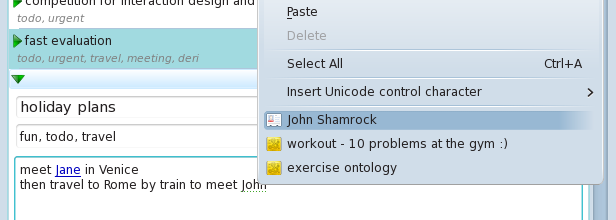
\includegraphics[width=\linewidth]{chapters/core/img/semnotes-screenshot-menu}
\caption{SemNotes annotation suggestion and link.}
\label{fig:annotation}
\end{figure} 

SemNotes does not currently offer suggestions based on online resources\footnote{Similar to \url{www.zemanta.com}.}, unless there is a desktop resource previously created for the relevant Web data (i.e. a bookmarked Web page becomes a desktop resource). 

We are working on an information extractor module, which identifies new information in the content of the notes. It will suggest the creation of new desktop resources from the text, like events, tasks or contacts, that will then be linked to the note. 

Since the annotation suggestions are computed while the user types the note, efficient processing is required. The process of finding possible matches follows:
\begin{enumerate}
 \item Scan the text and identify possible candidates represented by a single word or a sequence of words.
 \item For each possible entity found in the text find a list of existing desktop resources that match it. We use string matching to compute a score for each resource found. The score takes into account the length of the matched string, and if the resource has been linked to the note before.
 \item Sort the matches by score and present them to the user in a non-intrusive way (see Section \ref{sub:semnotesvisualization}).
 \item If the user chooses any of the presented suggestions 
  \begin{itemize}
   \item create a link between the piece of text identified as an entity and the actual resource it represents.
   \item use the selected suggestion in the recalculation of the scores for the entities found for the rest of the note. Once a note is linked to a resource, that resource is more likely to appear again, and therefore it will be ranked higher.
  \end{itemize}
 \item If the user ignores the presented suggestions, no links are created, but the possible matches are saved for later use.  
\end{enumerate}

For the purpose of establishing context, and for organising notes, it is sufficient to create a single link between a note and a resource it is related to, regardless of how many times that resource is mentioned in the content of the note. Therefore the relation between the note and the desktop resource is created only once in the repository. However, if the note is viewed in SemNotes, all the links that the user created to the related resource are displayed.

The interlinking module also manages the removal of links between notes and desktop resources.
Because the suggestion of related resources is based on the content of the notes, once the last textual link to a related resource is removed, so is the relation between the note and the respective resource. 

SemNotes also supports the manual creation of links between the note and desktop resources that are relevant but have no explicit mention in the text.

\subsection{Visualisation}
\label{sub:semnotesvisualization}

SemNotes displays the notes as a list that can be sorted by title, creation or last modification dates, or rating. Each note can be opened in-list for quick access, or maximised over the entire window, for viewing and editing. In the in-list mode, several notes can be open and edited at once (see Figures \ref{fig:screenshot} and \ref{fig:screenshot2notes} for the current version of the SemNotes user interface.).

\begin{figure}[tb]
 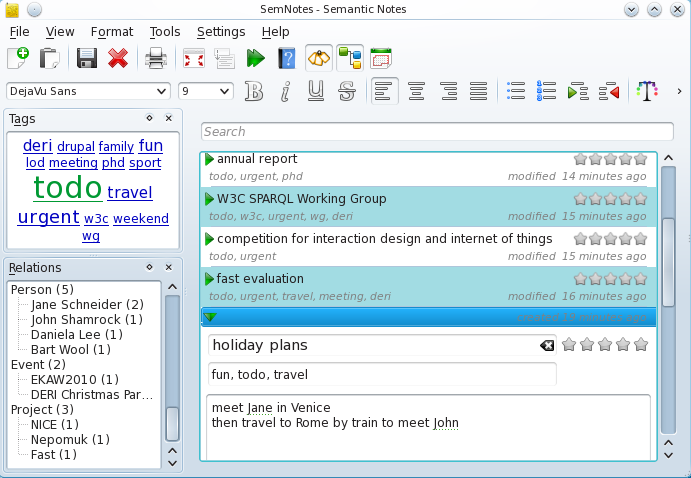
\includegraphics[width=\linewidth]{chapters/core/img/semnotes-screenshot}
\caption{Current version of the SemNotes user interface.}
\label{fig:screenshot}
\end{figure} 

\begin{figure}[tb]
 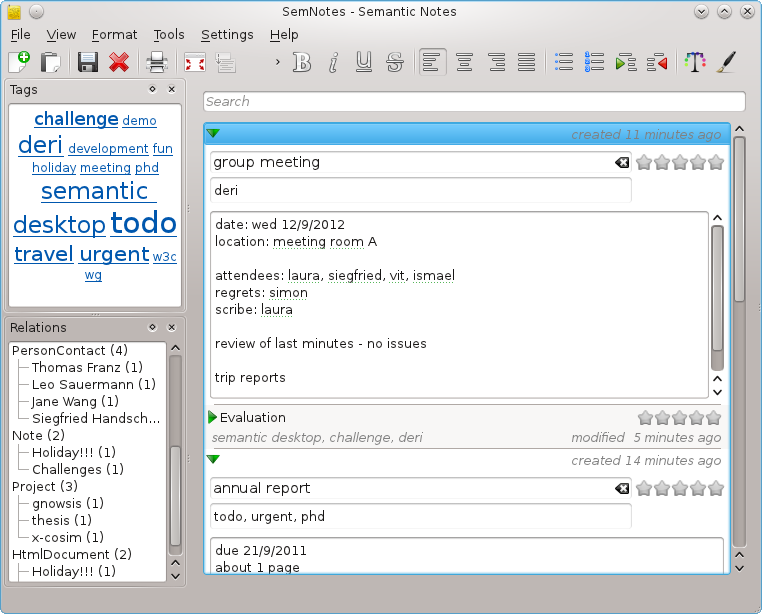
\includegraphics[width=\linewidth]{chapters/core/img/semnotes-screenshot_2notes}
\caption{SemNotes main window, with two notes open in-list.}
\label{fig:screenshot2notes}
\end{figure} 

An aggregated view of the list of notes is based on a restricted set of properties that the notes have in common. Depending on the set of properties used (one or more), the most suitable visual representation of the aggregated view varies. Currently SemNotes offers a tag cloud, a timeline and a related-resource view; each view aggregates information about the notes based on a single property (i.e. the tags associated, the creation date and the related resources, respectively). Aggregated views are displayed adjacent to the list of notes, and can be hidden by the user to allow more space for editing. 

These views also act as a custom faceted browser, as they provide filters on the list of notes. Filtering the list is as easy as clicking on a tag, time interval or related resource. A full text search box also acts as a filter on the list of notes, highlighting the search keywords in the content of open notes, if found. Multiple filters can be set at once, of mixed types. Figure~\ref{fig:screenshot} shows SemNotes with the tag cloud and related-resources views visible, and a tag filter set. A note is open in-list for editing. 

The editor component provides rich text editing of the note content, as well as easy editing of the note metadata. Tagging provides auto-completion based on all the tags on the Semantic Desktop, and creating a new tag is done just by typing its label. If the user does not set a title, SemNotes automatically sets it to the first line of the note. For the rating we used the default visualisation provided by the Nepomuk-KDE libraries, for a uniform interface across the desktop. The creation and last modification dates are the only metadata which cannot be changed through the user interface of SemNotes, as these properties are set automatically. They can be tweaked by expert users, by accessing the RDF repository directly. 

The suggestions for annotations are presented in a simple non-intrusive way, in the ``spell-checker'' style (i.e. the words for which suggestions were found are underlined with a green dotted line instead of a red squiggly line), and are available as context menu items, by right-clicking. Figure~\ref{fig:annotation} depicts how annotation suggestions are presented, and how a linked resource is displayed in the note. To remove an annotation is just as easy as creating it --- through a context menu item.

This presentation of the suggested resources is the result of several iterations of design, each improving on the previous one. 

\begin{figure}[tb]
 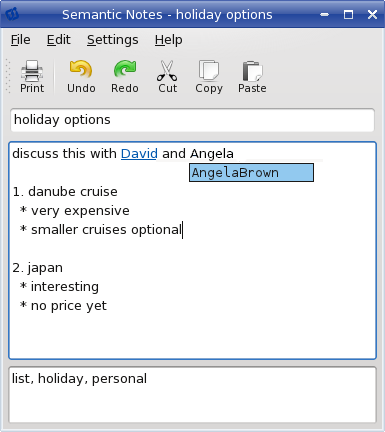
\includegraphics[width=0.6\linewidth]{chapters/core/img/linkednote_v1}
\caption{First version of the SemNotes note editor with pop-up style annotation suggestion.}
\label{fig:popup}
\end{figure} 

The first iteration relied on localised pop-ups with labels of the suggested resources, in the style of text auto-completion (see Figure \ref{fig:popup}). The style worked well when typing the text, and it also enhanced the speed of writing through the auto-completion it provided. The type of annotation of the text during its creation is called latent annotation \cite{Davis2010}, and it is an improvement over the two-step process of first creating the content and then annotating it. Depending on the text of the note, the pop-ups could appear often and distract the user, but they could be dismissed by continuing to type. However, when portions of text were pasted in the editor, several pop-ups were generated at the same time, which was confusing and did not allow the users to make all the connections they would. Changing slightly the pop-ups to only be displayed one-by-one when text was pasted proved not to be a good solution either, as in the case of large paragraphs it would take a long time and many mouse 
clicks for the paste operation to finish, thus interfering with the flow of work. 

Not just the interlinking support was changed from the first version of the application, but the entire user interface. The major redesign was supported by a usability study done as part of the Season of Usability\footnote{\url{http://openusability.org}} 2009, by Daivee Patel, a Human-Computer Interaction student at Drexel University, Philadelphia, USA, with the mentoring help of usability expert Paul Hibbitts of Hibbitts Design, Canada\footnote{\url{http://paulhibbitts.com}}. 
The goals of the project were to recommend changes to improve and/or redesign the SemNotes user interface based on analysis and user research methods, and to perform a usability evaluation of the new changes with a range of users to validate the design recommendations. 

The initial step of the project aimed at forming an understanding of what activities and tasks a user would perform with a note-taking application. This led to the use of a specific technique of task analysis called the activity grid based on the Activity Centred Design methodology. Using this method, we obtained a list of possible activities associated with using a note-taking tool, and each activity was subdivided into the tasks required to perform that activity and each task could then be further subdivided into possible actions. As the tasks became clearer, we identified the tasks that were relevant to SemNotes. These tasks helped focus the effort on the main usability issues and design specifically to address existing issues. 
A comparative analysis of five popular note-taking applications was conducted to help build a knowledge base for reference during the usability inspection of SemNotes. Each of the applications had their own unique features yet certain key functionality appeared standard across these kinds of applications. The examination proved helpful in determining the elements for redesign of the interface. 

The usability inspection of SemNotes was performed to identify usability issues with the existing interface that could be captured without the need to user test before the redesign.
Since the redesign was going to be based on key tasks or activities, we used a heuristic evaluation to identify top level issues.
The criteria for evaluation was the ISO standard ISO 9241\cite{ISO9241}, the principles associated with this standard are based on research and have the benefit of international consensus.
The results of the evaluation were used to help identify areas in the user interface most in need of design improvements, and to create a set of low fidelity mockups. 

A series of usability tests were conducted using the paper prototyping method to validate the initial recommendations for the interface redesign. During each testing session, participants were asked to think aloud and point to elements on the illustrated paper-based screen that they would click or look at based on the tasks provided. No assistance was provided to the users during the testing sessions. The usability test participants were selected via a screening survey on the criteria of experience with computer-based note-taking applications and note-taking habits. 
Based on the feedback from the first set of four users, the mockups were revised for the second round of usability testing while the tasks remained the same. The designs were further enhanced based on the 
feedback received in the second round. 

\begin{table}[htp]
\centering
\ra{1.3}
\begin{tabular}{p{0.45\linewidth} p{0.45\linewidth}}
\toprule
\textbf{Recommendation} & \textbf{Rationale} \\

\midrule
Multi Document Interface (presented as a single window with multiple panes) & By providing all key functionality within a single window, users did not have to manage multiple application windows.\\

Retain optional linking of text within linked editor via use of existing functionality (to click outside the auto complete pop-up) but to be supported by use of icons to indicate the type of resource being linked too & Users showed concern over unwanted text being linked. \\

Search should support searching by tags  & Users realised that since the notes were already tagged during creation, they would like to search by tags for better results. \\

Sorting of notes and tags in the left pane & Multiple options for sorting would help users in locating specific notes and/or tags. \\

First user experience should be provided & Learning curve associated with new applications -- having some introductory information and instructions in the opening screen will be useful. \\

\bottomrule
\end{tabular} 
\caption{Final recommendations for the redesign of SemNotes user interface, based on the usability study.}
\label{tab:sourecommendations}
\end{table}

Based on the accumulated results and feedback, we created a high fidelity mockup of the design, which included all the recommendations (see Table~\ref{tab:sourecommendations}) made as a result of the project, and which were incorporated in the second version of SemNotes.
The next iteration of the display for the annotation suggestions featured a side panel for each of the note edit boxes (see Figure \ref{fig:sidepanel}). The side panel proved to create less interference with the user's workflow, although the suggestions became less obvious. The panel presented the suggestions as a list of resources, that when clicked would highlight the parts of the content to which they were relevant. This helped the users understand from where the suggestion stemmed and if it was indeed correct. To create a link between the note and a suggested resource, the user had to right click on the corresponding item in the list and select ``Link''. Resources could also be removed from the suggestion list, and never be shown again for the current note, to help clear the list from overpopulating. This interface shifted the initial latent annotation style of SemNotes, back to a classic two-step process. Although the suggestions were still computed on the fly, as the user typed or pasted new text, 
because they were out of focus, users were inclined to leave the annotation step for later. Another issue of the side-panel variant was that it limited the screen real-estate for the most important function of SemNotes, that of note-taking. 

\begin{figure}[tb]
 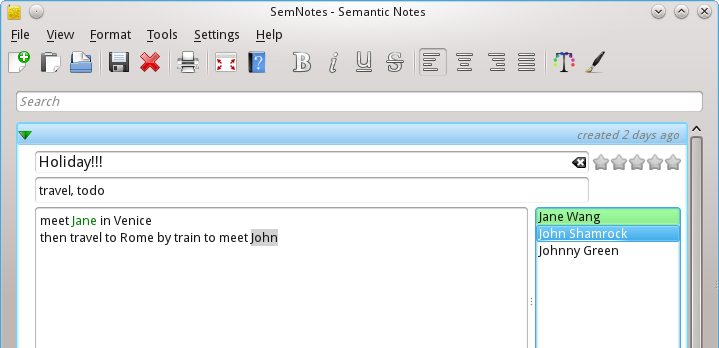
\includegraphics[width=\linewidth]{chapters/core/img/linkednote_v2}
\caption{Second version of the SemNotes note editor with a side panel to display the annotation suggestions.}
\label{fig:sidepanel}
\end{figure} 

To keep more of the screen space for the note editor, in the next iteration, we have abandoned the side panel in favour of the ``spell-checker'' type of notification. It is a mix of the first and second iterations, by giving the users the immediate feedback of the pop-ups, through the green dotted line that underlines words, while being unobtrusive in the note-taking activity. The suggestions are computed on-the-fly like before, but they are only shown if the user right-clicks on the underlined word or words, in keeping with the spell-checker metaphor.

The three iterations of user interface design have improved significantly the usability of SemNotes, as well as the ease of interlinking. However, further usability testing is needed to determine whether and how different types of relations can be created between the notes and the related desktop resources. 


\section{Evaluation}
\label{sec:semnotesevaluation}

We conducted a task-based summative user evaluation, comparing SemNotes to the popular note-taking application Evernote\footnote{\url{http://evernote.com/}}. The goal of the experiment was to determine whether the effort required for the creation of links between notes and resources is repaid by easier search. Towards this goal, we measured the effort needed to execute the same set of tasks with both tools, and compared the results. We used time spent, number of mouse clicks and number of key presses, as measures for effort. After the experiment, we asked the participants about their experience in a questionnaire.

The two applications compared have the same main functionality, note-taking. We chose Evernote as baseline, as it is a very popular note-taking tool that is freely available. Its set of functionalities are richer than those of SemNotes, but the basic features are present and similar in both applications. The feature that distinguishes SemNotes is the same that we want to measure---the creation of links between the notes and desktop resources, based on suggestions given by the application. SemNotes runs on KDE on Linux, and uses the framework provided by Nepomuk-KDE Semantic Desktop. Evernote runs on several operating systems for desktop and mobiles, but Linux is not one of them, therefore we used its Windows version. 

Evaluation is one of the challenges for application design on the Semantic Desktop. Adding to the challenges of evaluating PIM applications with regards to finding appropriate data and tasks for significant measurements, discussed in \cite{Kelly2006}, semantic PIM applications have the difficulty of lacking equivalent semantic tools for a one-on-one comparison. That is why for this evaluation, we followed a methodology similar to the ones described in \cite{Elsweiler2007} and \cite{Franz2009}, of comparing our semantically enabled SemNotes, to a conventional application.

One aspect that we did not evaluate as part of this study is the effect of having the notes connected to the relevant desktop resources from the other applications using the respective resources --- for example, would the extra information from the notes provide an advantage when using a task manager application, and seeing all the linked notes when looking at a task. Such a study would require a longer duration, and also a richer ecosystem of semantic applications, which make use each other's data.

\subsection{Participants} 

Twenty participants took part in the evaluation, all members of our research institute. They are researchers in the field of Semantic Web, thus possibly favouring the semantic application. This bias (if it exists) would however influence only their responses in the questionnaire and not the measured values. Fourteen participants regularly use note-taking and five of them use Evernote as their preferred note-taking tool. None of the participants used Linux as their operating system. Their familiarity with one environment and one application could have influenced the measured results, in favour of Evernote.

\begin{figure}[htb]
 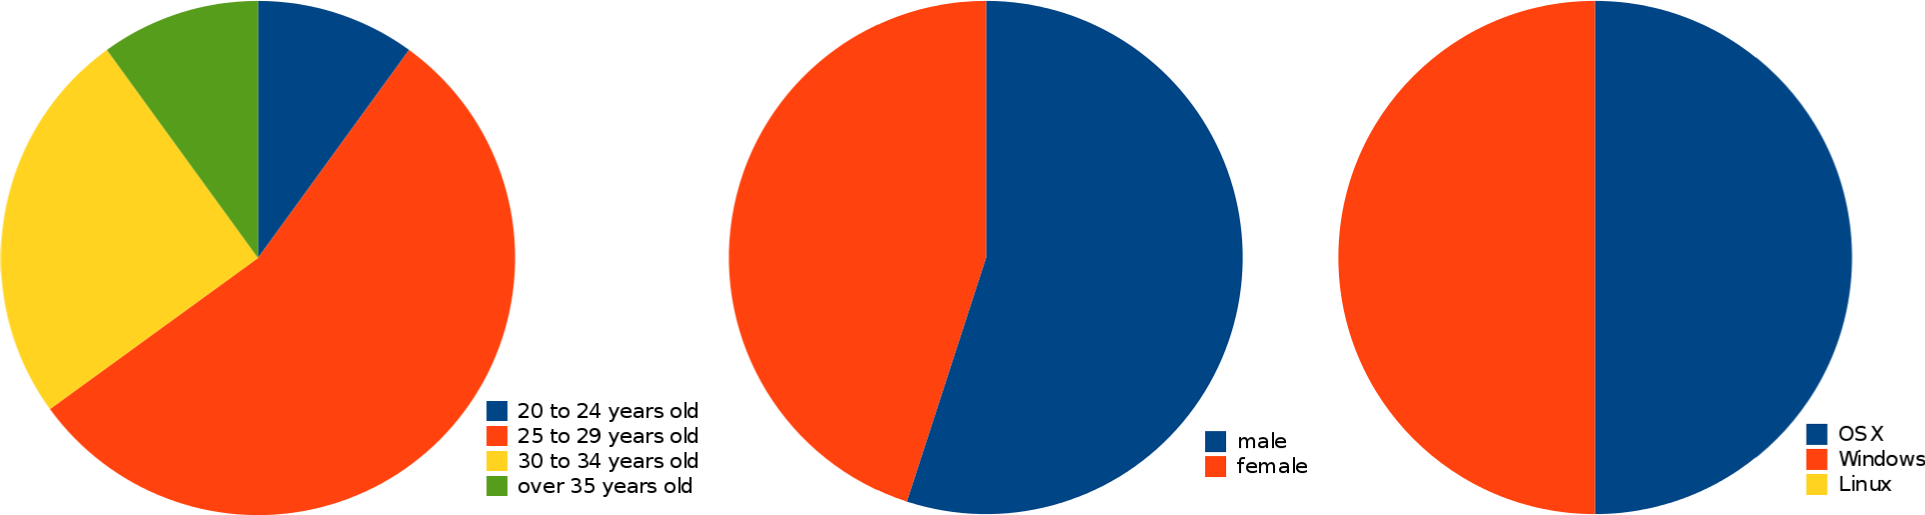
\includegraphics[width=0.95\linewidth]{chapters/core/img/distribs}
\caption{Age, gender and OS distributions of participants.}
\label{fig:distribs}
\end{figure}

Some additional demographic details of the participants: gender distribution was close to even (eleven men and nine women); most of them were in the age groups between 25 and 29 (eleven, equivalent to 55\%), and between 30 and 34 (five, or 25\%). There were seven Master's students, seven Ph.D. students, five senior researchers and one intern. For demographic distributions see Figure \ref{fig:distribs} and Figure \ref{fig:genderdistribs}.

\begin{figure}[htb]
 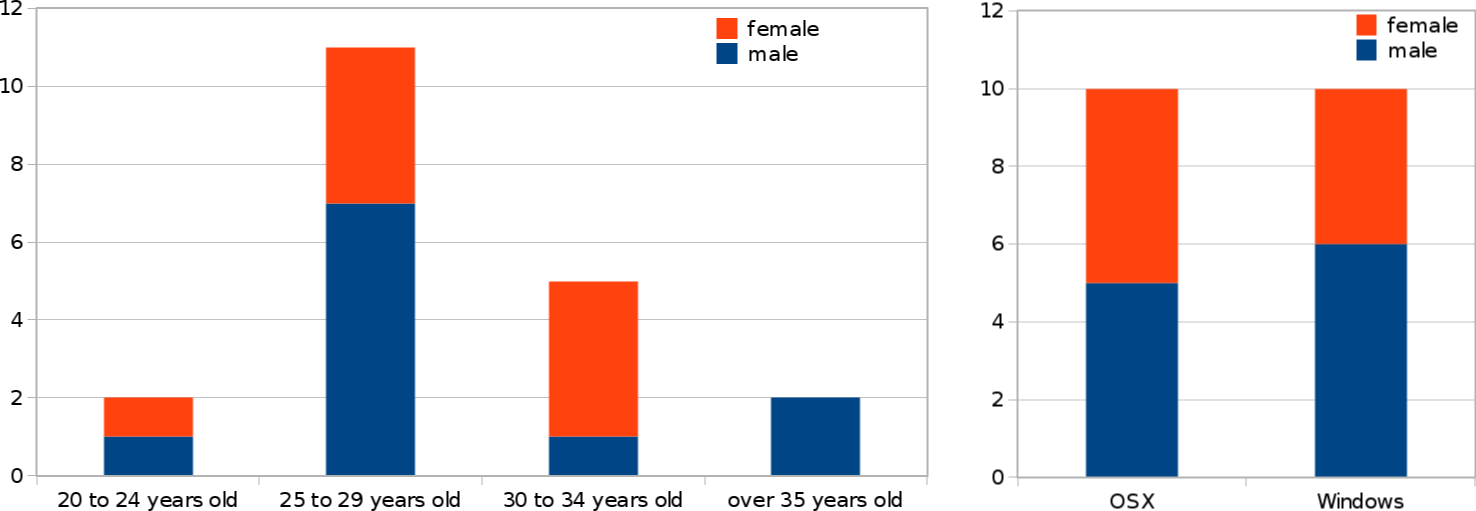
\includegraphics[width=0.9\linewidth]{chapters/core/img/genderdistribs}
\caption{Age and OS distributions of participants per gender.}
\label{fig:genderdistribs}
\end{figure}

\subsection{Data} 

We used two virtual machines for the experiment, preloaded with identical data. To reduce the artificialness of the study, we chose general data familiar to the participants, to which they have access in their everyday work. The dataset contained contact information for 130 members of our institute; 655 recent emails from our mailing lists; 20 scientific papers authored by our colleagues; and photographs from institute events. The note data was also identical: 50 notes on a variety of topics, personal or work-related, tagged with 23 tags. In SemNotes, we also provided links between the notes and the resources mentioned in them: people, projects, events or other notes, within reasonable limits we expect users to interlink their notes (i.e. minimum 0 links, maximum 10 links, average 1.8, median 1). The majority of connections were made to people mentioned in the notes.

\subsection{Tasks} 

We prepared a set of eight tasks. Each participant was requested to run all the tasks in each of the two environments. To prevent order effects from influencing the results, half of the participants started with SemNotes and the other half with Evernote.

\begin{description}
 \item[T1.] Find what information is available about yourself (contact information, documents, emails, photographs)
 \item[T2.] Find the paper titled ``Bridging the Gap between Linked Data and the Semantic Web''. Who are the authors?
 \item[T3.] Find notes tagged with ``todo''.
 \item[T4.] Find to-dos that are related to our institute.
 \item[T5.] Find a to-do related to a presentation by a colleague John.
 \item[T6.] Take a note about planning a social event for your research group. Write the names of two people that have already confirmed. Annotate the note as you see fit.
 \item[T7.] Find a note containing the minutes from the last meeting about a given project. Change the date of the next meeting planned.
 \item[T8.] Take a new note for the action item assigned to you at the last meeting of the project. The action item is in the meeting minutes previously edited, and it requires drafting a document using a paper authored by a colleague. Annotate the note.
\end{description}

The first two tasks were intended to help the participants get accustomed with the data available and the environment; we did not include the time spent on these tasks in the results. 

The last six tasks were focused on note-taking, and their complexity increased gradually. T3, T4, and T5 are search and filter tasks (S), from the very simple to the complex. T6 and T8 are editing tasks (E), including any annotations that the participants made on the notes. T7 is both a search and edit task (SE). It prepares the participants for the most complex search and edit task, T8, which required interaction with the rest of the system (i.e. finding the required paper).

\subsection{Measurements} 

The participants were recorded while doing the tasks of the experiment, and the videos were used to extract the measurements used in the analysis. 
For each task we measured the effort in seconds spent, and number of mouse clicks. 
We also counted the number of key strokes for the tasks involving creation of notes, and we used this measure to normalise the values for time. 
Although we had two separate measures for each task, we were interested in the difference between these values, computed according to:
$$
value_{difference} = value_{SemNotes} - value_{Evernote}
$$
Thus, a positive value means that the value recorded for SemNotes is bigger than the corresponding value for Evernote, and a negative value means that the value for SemNotes is smaller. 

For the time measurements, the time difference represents the extra \emph{effort} required for annotating the notes with links in the editing tasks. For the search tasks the difference shows which of the applications enables the users to find the notes easier, thus the \emph{benefit}. We must specify here that actual searches done by the software were considered instantaneous, as the datasets are small and we did not intend to measure the performance of the search algorithms used.

For the number of mouse clicks, the difference represents the extra \emph{effort} required, for both types of tasks.

\begin{figure}[tb]
\begin{center}$
 \begin{array}{ccc}
  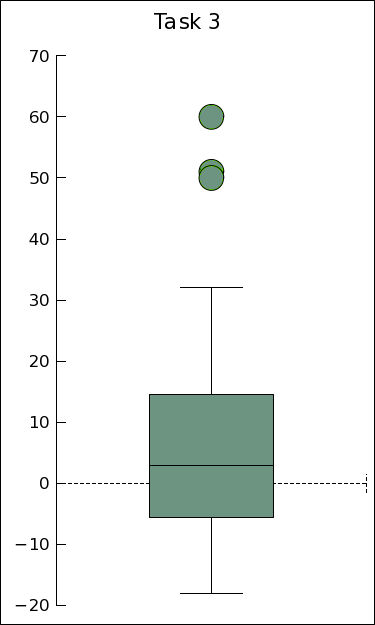
\includegraphics[width=0.29\linewidth]{chapters/core/img/task3difboxplot} &
  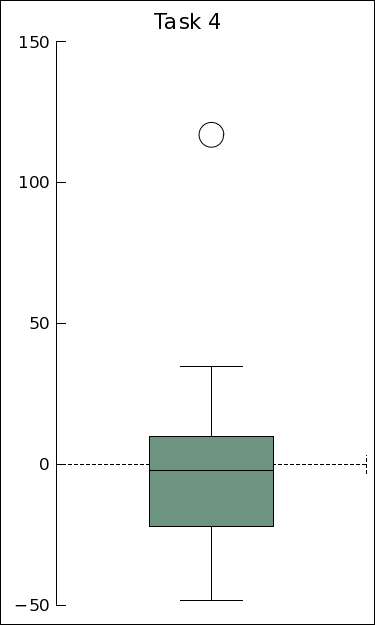
\includegraphics[width=0.29\linewidth]{chapters/core/img/task4difboxplot} &
  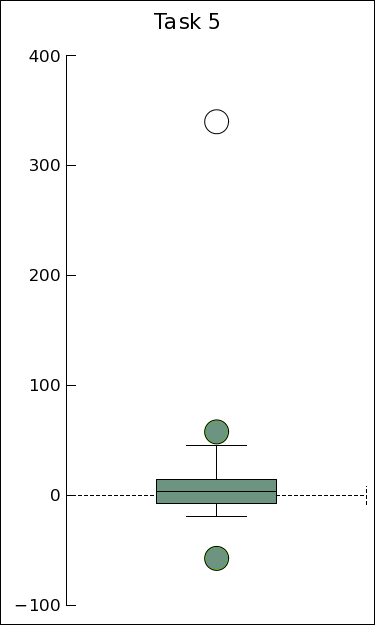
\includegraphics[width=0.29\linewidth]{chapters/core/img/task5difboxplot} \\ 
  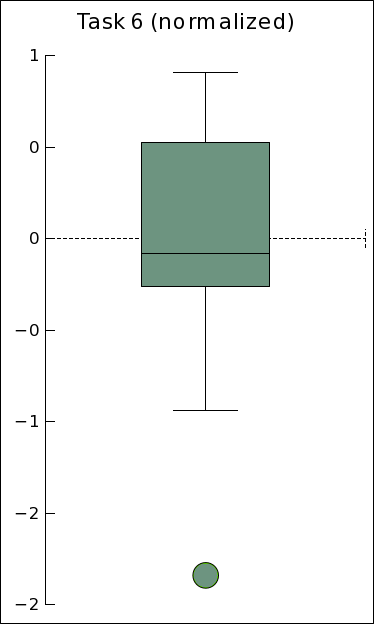
\includegraphics[width=0.29\linewidth]{chapters/core/img/task6difboxplot} &
  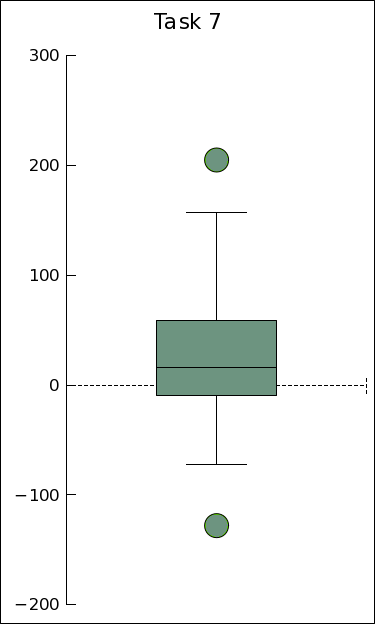
\includegraphics[width=0.29\linewidth]{chapters/core/img/task7difboxplot} &
  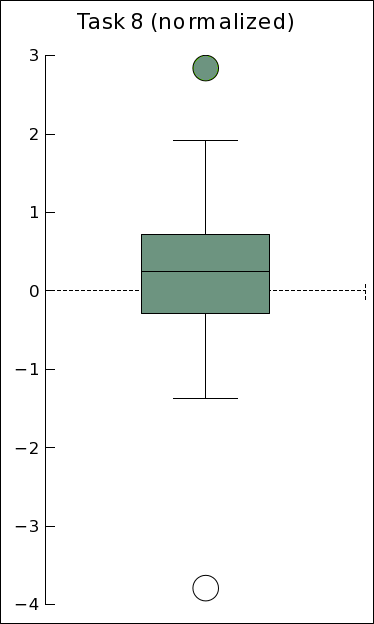
\includegraphics[width=0.29\linewidth]{chapters/core/img/task8difboxplot} 
 \end{array}$
\end{center}
\caption{Inter-quartile ranges for the time difference.}
\label{fig:boxplots}
\end{figure}

After a first analysis of the results, we noticed that some values for time were unrealistically high or low. They coincided with the measurements when the participants stopped to ask a question or comment on a feature. We decided to eliminate these outlier values by using only the measurements that fall in the inter-quartile range, for all tasks --- see Figure \ref{fig:boxplots}.

\subsection{Quantitative Results}

We tested if the effort measured in time and mouse clicks was different when using SemNotes than when using Evernote. Table \ref{tab:semnotesresults} shows the results, with the statistically significant values in bold (\begin{math}p < 0.05 \end{math}).

\begin{table}[htp]
\centering
\ra{1.3}
\begin{tabular}{@{}clcr@{.}lr@{.}lr@{.}lcr@{.}lr@{.}lr@{.}l}
\toprule
\multirow{2}{*}{\textbf{T}} &&& \multicolumn{6}{c}{\textbf{Time (s)}} && \multicolumn{6}{c}{\textbf{Clicks}} \\

&&& \multicolumn{2}{c}{\textbf{Avg}} & \multicolumn{2}{c}{\textbf{Med}} & \multicolumn{2}{c}{\textbf{\textit{t}}} && \multicolumn{2}{c}{\textbf{Avg}} & \multicolumn{2}{c}{\textbf{Med}} & \multicolumn{2}{c}{\textbf{\textit{t}}} \\
\midrule
\textbf{T3} & (S) && 0 & 5 & 0 & 0 & 0 & 152 && 0 & 167 & 0 & 0 & 0 & 692 \\

\textbf{T4} & (S) && -8 & 0 & -8 & 0 & \textbf{-2} & \textbf{94} && -0 & 333 & -1 & 0 & -0 & 48 \\

\textbf{T5} & (S) && -0 & 125 & 1 & 0 & -0 & 046 && 0 & 857 & 1 & 0 & 1 & 426 \\

\textbf{T6} & (E) && 0 & 063 & 0 & 016 & 0 & 486 && 6 & 067 & 8 & 0 & 2 & 026 \\

\textbf{T7} & (SE) && 14 & 357 & 13 & 0 & 1 & 713 && 4 & 812 & 2 & 0 & 1 & 527 \\

\textbf{T8} & (SE) && 0 & 249 & 0 & 243 & 1 & 004 && 20 & 8 & 12 & 0 & \textbf{3} & \textbf{08} \\

\bottomrule
\end{tabular} 
\caption{Statistics for time and click differences.}
\label{tab:semnotesresults}
\end{table}

Results show that for the simple search task T3 the difference is positive, which suggests that it takes longer to finish the task with SemNotes. However, the difference is not significant. For the complex search tasks that follow, T4 and T5 the difference has negative values, showing that the users spent less time on complex searches when using SemNotes, thus supporting the claim that the use of interlinked data makes notes easier to find. Only the results for T4 are statistically significant. None of the measures of number of mouse clicks for the search tasks are statistically significant, the differences being in average less than 1 click, with a median value of 0, -1 and +1 respectively for the tasks T3, T4 and T5.

For the editing task T6, the values are positive, thus it took longer to finish it with SemNotes. This was expected, as in SemNotes there is the additional step of annotating the notes with links to desktop resources. However, the differences are very close to 0 (0.063s average and 0.016s median) and not statistically significant. This editing task did require in average 6 more mouse clicks in SemNotes, with a median value of 8, but the difference is also not statistically significant.

For the more complex search and edit tasks T7 and T8, the time differences, while positive, thus in favour of Evernote, are not significant. For both tasks the values were positive, which mean more clicks when using SemNotes. However, task T8, that required creating and annotating a complex note based on information from other sources, had statistical significant difference in number of clicks, in favour of Evernote (more clicks needed in SemNotes). 

The positive difference in the number of clicks required for all editing tasks (T6, T7 and T8) is not surprising, as the participants recognised the value of creating links and proceeded to link the new note to the relevant resources. This was however a motivation for providing better keyboard support for the annotation of notes in the future version of the tool.

In summary, the results show that there are significant improvements (for one of two tasks) in the time spent on complex searches, when the data is interlinked, at no significant extra cost for the creation of the links. Linking does however significantly increase the effort measured by number of mouse clicks (for one of two tasks).

\subsection{Questionnaire}

We asked the participants to fill in an anonymous questionnaire related to the experiment. The questionnaire is listed in Appendix~\ref{ap:questionnaire}. According to the answers, on a scale from 1 to 5, the tasks were simple (mean 2.25) and similar to the ones in their daily work (mean 3.4), and the data provided was familiar (mean 3.2). 

The answers also show that 60\% of the participants (12) felt that SemNotes helped them finish the tasks \emph{faster}, while only 20\% (4) said Evernote, and 20\% did not feel any difference between the tools. When asked which of the two applications helped them perform the tasks \emph{better}, 80\% of the participants chose SemNotes, while the remaining 20\% did not feel that there was any difference (see Figure \ref{fig:betterfaster} for a graphical representation).

\begin{figure}[htb]
 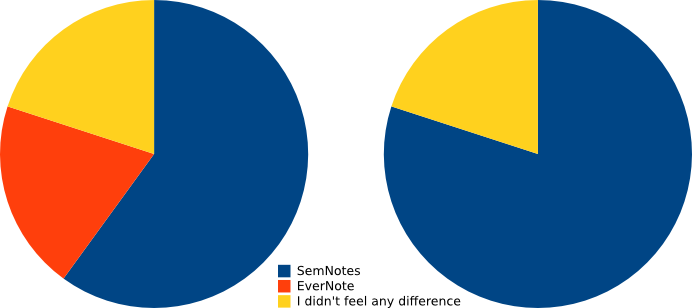
\includegraphics[width=0.7\linewidth]{chapters/core/img/fasterbetter}
\caption{Which tool helped perform the tasks faster (left) and better (right).}
\label{fig:betterfaster}
\end{figure}

The participants had a good overall impression of SemNotes (with a mean of 4.15 on a scale from 1 to 5). This rating was supported by comments like ``\emph{That was cool.}'', and requests for SemNotes for other operating systems: ``\emph{Maybe you could make an OS X version?}'' and ``\emph{When is a port for Windows 7 coming?}''.

The semantic annotation was one of the most liked features of SemNotes, and one of the features most missed in Evernote, according to the questionnaire. Another advantage of SemNotes was considered the multiple filtering by mixed criteria, with several participants considering it the best feature. The rating of notes was listed as the least liked feature of SemNotes by three participants. The tag cloud was the most controversial feature, as many participants liked it and found it very useful, while others would have preferred a simple list of tags: ``\emph{Usually I don't like tag clouds, but the one in SemNotes was really useful.}'' and ``\emph{While the tag cloud helps in determining the most used tag, a simple list with the tags seems to be easier to search.}'' 


\section{Related Work}
\label{sec:notetakingapps}

Semantic note-taking means enhancing the note-taking process using Semantic Web technologies. It can refer to the techniques and methods used in the implementation, like ontologies and RDF, but most importantly it is about creating a semantic network around the notes and the information contained in them. There are several applications that enable more or less semantic note-taking: some are browser based (online or offline), while others are standalone desktop applications as is SemNotes. 

The List.it browser-based note-taking tool \cite{Kleek2009} and Jourknow, its predecessor \cite{Kleek2007}, save context alongside the information scraps, to improve re-finding and reminding. List.it also features information extraction from the unstructured text of the notes, recognising entities and relations between them, with the \emph{pidgin} language processor. However, unlike SemNotes, the contex of the notes they create does not include links to any existing desktop resources. SnapShoot \cite{Iga2006} is another browser-based note-taking tool that explores new visualisation techniques to improve reading of the documents produced. It features categorisation, and limited interlinking with documents within the system.

MindRaider \cite{MindRaider}, described above in Section \ref{sec:sdsystems}, is an open source ``Semantic Web outliner'' and extended note-taking system for information organisation. While it only interlinks concepts within its maps, it can connect to the Gnowsis Semantic Desktop through a plugin, thus potentially it can use any Semantic Desktop resources through a similar mechanism.

A distinct category of semantic note-taking applications are personal semantic wikis, like Kaukolu \cite{Elst2008}, IkeWiki \cite{Schaffert2006} and GDKTiddlyWiki. Each wiki page represents a resource and its semantic relations to other resources are encoded within the page, using an extension to the wiki syntax. Only predefined relations and types are available, and the wikis offer limited access to other desktop information sources. Unlike SemNotes, connections are only possible between resources within the wiki system.

OneNote from Microsoft's office suite provides quasi-se\-man\-tic functionality by interlinking the notes with address book information, calendar, and tasks. It does not use any semantic technologies though, and the data is locked in by proprietary formats and storage.

Zemanta\footnote{\url{http://www.zemanta.com}} is a blog assistant that suggests possible enhancements to blog posts, like linking external content and images. Unlike SemNotes, which uses the local repository to search for matches, Zemanta looks on the Web. It does not assign any semantics to the links. 

There are also specialised systems like the SemanticPen \cite{Varadarajan2005} which provides support for semantic note-taking with pen devices.
Other note-taking applications that provide semantic features include: Jenga Note\footnote{\url{http://www.jenganote.org}} --- allows associating a note with a concept, Catch Notes\footnote{\url{http://www.catch.com}}, and SpringPad\footnote{\url{http://www.springpadit.com}}.


\section{Conclusion}

In this chapter, we presented a solution to the challenges of designing applications for the Semantic Desktop. We described one such application, SemNotes, a semantic note-taking tool for the Nepomuk-KDE Semantic Desktop. It provides a real-world, functional use case for fully exploiting the capabilities of the Semantic Desktop: interlinking, organisation and management of personal information, efficient search and browsing. It supports the entire life-cycle of the semantic data represented by notes, with emphasis on the creation of links between the new data and the existing network of linked information on the desktop. 

Through SemNotes we present a possible solution to each of the challenges presented in the begining of the chapter. To the first question of creating semantic data, we describe how we create new semantic notes, using the existing vocabularies and creating links to the existing Semantic Desktop data available. To the second question of designing the human computer interaction, we describe the efforts towards an easy to use yet rich user interface design for SemNotes. With the help of usability experts and user testing the interface went so far through three iterations, each described in this chapter.

For the third challenge, that of evaluating a semantic tool, we described a task-based user evaluation comparing SemNotes to the popular note-taking application Evernote. The results show that the extra effort (measured in time spent) required for the annotation of notes with links to related resources is not significant. However, the benefit (measured in time saved) is significant for one of two complex search tasks. 

SemNotes embodies a simple and user-friendly way of generating new semantic data on the desktop, and integrating it with the already existing data. However, the personal information that the users work with is not restricted to the desktop. Further, semantic data exists in large quantities outside of the desktop, on the Web and in organisational repositories. Thus, in the next chapter we continue by describing how the linked information from the desktop can be meaningfully and safely connected to the outside world.
